\documentclass{article}
\usepackage[utf8]{inputenc}
\title{MapReduce: Simplified Data Processing
on Large Clusters}
\author{wbg231 }
\date{December 2022}
\newcommand{\R}{$\mathbb{R}$}
\newcommand{\B}{$\beta$}
\newcommand{\A}{$\alpha$}
\newcommand{\D}{\Delta}

\newcommand{\avector}[2]{(#1_2,\ldots,#1_{#2})}
\newcommand{\makedef}[2]{$\textbf{#1}$:#2 }
\usepackage{tikz,graphicx,hyperref,amsmath,amsfonts,amscd,amssymb,bm,cite,epsfig,epsf,url}

\begin{document}

\maketitle

\section*{abstract}
\begin{itemize}
\item \href{https://brightspace.nyu.edu/content/enforced/261985-SP23_DS-GA_1004_1_001/p107-dean.pdf}{paper link}
\item \href{https://www.youtube.com/watch?v=cvhKoniK5Uo}{Computerphile video }
\item map reduce is a programming model and associated implementation for processing and generating large data sets that is good for real world tasks
\item users specifies quires in terms of a map and a reduce function and the under lying run time system atomically paralyzes computation across numerous machines, 
\item pretty widely used at good 
\section{introduction}
\item this was written to deal with large quantities of data, and allow for code that is easily parallelization 
\item abstraction allows computations to be expressed while hiding the details of parallelization, 
\imte based on the MP and reduce primitives in many functional programming languages
\item most computations involve applying a map operation to each record in the input in order to compute a set of key/value pairs, then applying a reduce operation to all the values that shared the same key in order to combine the derived data appropriately  
\item using the map and reduce abstraction allows for easy parallelization
\section{programming model}
\item the computation takes as input a set of key values pairs and produces as output a set of key values pairs
\item the user expresses the computation into terms of two functions a map and reduce function
\item map written by the user takes an input pair and produces a set of intermediate key/value pairs. 
\item the map reduce library groups all intermediate key values associated with the same intermediate keys and passes them to the reduce function 
\item the reduce function written by the user accepts an intermediate key I and a set of values fro that key, it merges these values together to form a new set of values. 
\item the intermediate values are supplied to the user reduce function via an iterator allowing sets of value too large to be read into memory to be handled 
\subsection{example}
\item suppose we want to find the number of occurrences  of each word in a large collection of documents 
\item pseudo code for map and reduce function \\ 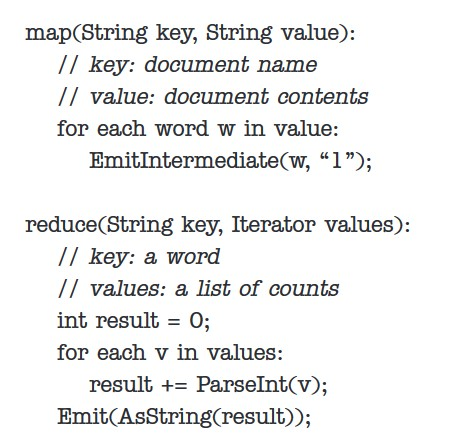
\includegraphics[width=5cm]{reading assignment notes/week 2/MapReduce: Simplified Data Processing on Large Clusters/images/mw_1.jpg} 
\item the map function outputs each word and an associated count of occurrences. 
\item the reduce function sums all counts of each word
\subsection{types}
\item map$(k_1, v_1)\rightarrow list(k_2,v_2)$
\item reduce $(k_2, list(v_2))\rightarrow list(v_2)$
\item meaning the input keys and values are drawn from different domains than the output keys and values. the intermediate keys and values are from the same domain as the output key and value 
\item so in the example input key is a document name value is its content. 
\item the intermediate keys are a word and the value is the number of occurrences of the word in a single document 
\item then the output keys are a word and the output values are the number of occurrences of that word across all documents 
\section{implementation}
\item the correct implementation is domain specific, but they are going to go over how the one at Google is implemented 
\subsection{execution overview}
\item map invocations distributed across multiple machines by portioning the input data into a set of M splits 
\item the input splits can be processed in parallel by different machines 
\itme reduce invocations are distributed by portioning the intimidated key space into R pieces using a portioning function.  (so that is for instance if there are 100 words, each of 10 computers runs the reduce function on intermediate key value pairs for the 10 of the 100 words) 
\item execution order 
\begin{itemize}
    \item input files split into M pieces. many copiers of program started across the cluster of machine
    \item one special copies of the program called the master assign work to the other copies of the program called the workers .there are M map tasks and R reduce tasks to assign 
    \item a worker assigned a map task reads the content of the corresponding input split. parses key/value pairs of the input data and passes each pair into the par function. the intermediate key value pairs produced by the map function are buffed into memory.
    \item periodically buffed pairs are written to the local disk, portioned into R regions by the part ion function. the locations of these buffed pairs on the local disk are passed back to the master who is responsible for forwarding these locations to the reduce workers .
    \item when a reduce worker is told about the location it uses remote procedure class to read the buffered data from the local disk of the map workers, when a reduce worker has read all the intermediate data for its partition it sorts it by the intermediate keys so that all occurrences of the same key are grouped together then sorting is needed many different keys map to the same reduce task. if the amount of intermediate data is too large for memory an external sort is used 
    \item the reduce worker iterates over the sorted intermediate data and for each unique intermediate key encounters passes the key and the corresponding values to the user defined reduce function. the output of the reduce function is appended to a final output file for this reduce partition 
    \item when all map and reduce tasks have been completed the master wakes up the user program at returns back to the user code 
\end{itemize}
\item map reduce diagram \\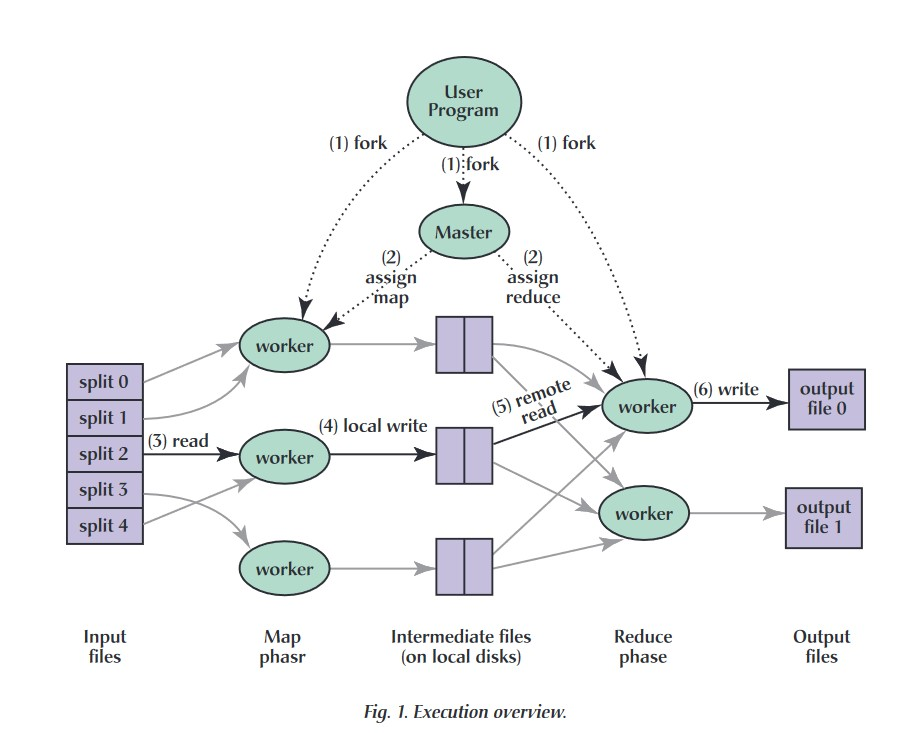
\includegraphics[width=5cm]{reading assignment notes/week 2/MapReduce: Simplified Data Processing on Large Clusters/images/mw_2.jpg} 

\subsection{master data structures}
\item the master keeps track of the state (idle, in progress, complete) of each worker as well as the identity of each worker machine 
\item the master also stores the location and size of ht intermediate file produced by the map task
\item i think i have the large scale picture of this paper, the rest is really technical details and performance information so i am going to skip it for now. 

\end{itemize}
\end{document}
